% Template for WHISPERS-2009 paper; to be used with:
%          stywhispers.sty  - WHISPERS LaTeX style file, and
%          IEEEbib.bst - IEEE bibliography style file.
% --------------------------------------------------------------------------
\documentclass{article}
\usepackage{spconf,amsmath,epsfig}
\usepackage{algorithm2e}
\usepackage{algorithmic}
\usepackage{amssymb}
\usepackage{hyperref}
\usepackage{xcolor}
\usepackage[font=scriptsize,labelfont=scriptsize]{subcaption}


% Example definitions. 


% --------------------
\def\x{{\mathbf x}}
\def\hx{{\hat x}}
\def\L{{\cal L}}
\def\R{{\mathbb R}}
\def\E{{\mathbb E}}
\newcommand{\Dt}{\mathcal{D}_{t}}
\DeclareMathOperator*{\argmax}{arg\,max}
\DeclareMathOperator*{\argmin}{arg\,min}
\newcommand{\JMM}[1]{{\textcolor{blue}{[#1]}}}


% Title.
% ------
\title{Deep Diffusion Processes for Active Learning of Hyperspectral Images}
%
% Single address.
% ---------------
\name{Duc Nguyen, Abiy Tasissa, James M. Murphy} 
\address{Department of Mathematics, Tufts University, Medford, MA 02155, USA
	}


\begin{document}

\maketitle

\begin{abstract} A method for active learning of hyperspectral images (HSI) is proposed, which combines deep learning with diffusion processes on graphs.  A deep variational autoencoder extracts smoothed, denoised features from a high-dimensional HSI, which are then used to make labeling queries based on graph diffusion processes.  The proposed method combines the robust representations of deep learning with the mathematical tractability of diffusion geometry, and leads to strong performance on real HSI.  

\end{abstract}

\begin{keywords}hyperspectral images, variational autoencoders, deep clustering, active learning, diffusion geometry\end{keywords}

\section{Introduction}
\label{sec:Introduction}
 
 Machine learning has provided revolutionary new tools for remote sensing, but state-of-the-art methods often require huge labeled training sets.  In particular, supervised deep learning methods can achieve near-perfect labeling accuracy on high-dimensional hyperspectral images (HSI), provided huge libraries of labeled pixels are available \cite{Zhu2017_Deep}.  This hinders the practicality of these methods, as in many settings, data is collected at a pace that far exceeds human ability to generate corresponding labeled training data.
 
 In order to account for this, methods that require only a very small number of labels are needed.  The \emph{active learning} regime is particularly attractive for HSI labeling problems.  In active learning, an algorithm is provided with an unlabeled dataset, and the algorithm iteratively queries points for labels.  By choosing query points in a principled manner, the resulting parsimonious training set can provide the classification performance of a much larger training set chosen uniformly at random.  
 
 We propose an active learning method for HSI based on deep feature extraction and random walks on graphs.  A variational autoencoder is used to nonlinearly denoise and compress the high-dimensional HSI.  Then, the resulting features are considered as vertices of a graph, and a Markov diffusion process on the graph is used to determine label queries and label all data points.  The proposed method combines the excellent feature learning of deep autoencoders with the mathematical interpretability of graph diffusion processes, and leads to strong empirical performance on real HSI.  

%%%
%%%

\section{Background}
%We propose an active learning algorithm which has two main stages. The first stage is feature extraction of an unlabeled high-dimensional dataset using a variational autoencoder. The second stage employs an active learning diffusion based clustering algorithm to infer the true labels. In what follows, we describe these two stages in detail. 
Extracting essential features of data is an important part of both supervised and unsupervised machine learning problems. For example, the unsupervised technique of Gaussian mixture models (GMM) assumes that the data under consideration is an i.i.d. sample from a mixture of Gaussians. To solve the unsupervised clustering problem on these data, parameters of the GMM are then estimated using the expectation maximization algorithm \cite{Murphy2012_Machine}. In recent years, deep generative methods, such as \emph{generative adversarial network (GANs)} and \emph{variational autoencoder networks (VAEs)}, have been used as feature extraction tools and successfully applied to many machine learning tasks \cite{ehsan2017infinite,makhzani2015adversarial}. In the context of the clustering problem, a set of methods, known as deep clustering, propose learning features of the data and clustering simultaneously, showing strong empirical results \cite{tian2014learning,song2013auto,xie2016unsupervised,jiang2017variational}. 
\subsection{Variational Autoencoder Networks (VAEs)}


We now describe VAEs following the exposition in \cite{yang2018geodesic}. Let $x \in \R^N $ and consider a latent variable model $p_{\theta}(x) = \int p(x|z)p(z)\,dz$. The variable $z\in \R^{k}$, $k\ll N$, is a latent variable and provides a low-dimensional parametrization of the data $x$. The goal of VAE is to maximize the probability of  data samples generated as $p(x)$. In the inference part of VAE, the training procedure maps a data point $x$  to its latent representation $z$ such that the $z$ adheres to the distribution $p(z)$. 

Since the posterior distribution $p(z|x)$ and $p(z)$ are unknown, VAE makes the assumption that $p(z|x) = q(z|x,\phi)$ where $\phi$ \JMM{where does $\phi$ live?} are parameters to be learned from the network. To enforce that the variational distribution $q(z|x,\phi)$ agrees with $p(z)$, the optimization \[\min_{\phi}\,\, KL(q(z|x,\phi),p(z)),\] is considered, where KL is the Kullback-Leibler divergence.  With this, $q(z|x)$ can be interpreted as the encoder part of VAE providing us a latent representation $z$ given a sample $x$. The generative part of VAE considers the reconstruction of a data sample given the latent representation $z$. In particular, the goal of the training procedure is to map a latent variable $z$ to a data sample $\hat{x}$ such that $\hat{x}$ is similar to the true data sample $x$. This naturally motivates the maximization of $p(x|z,\theta)$ with $\theta$ denoting the network parameters. Formally, we consider the following optimization program:
\[
\max_{\theta}\, \E_{z \sim q(z|x,\lambda)} \log(p(x|z,\theta))
\]
With this, $p(x|z)$ can be interpreted as the decoder part of VAE. The inference and generative parts of VAE i.e the encoder and decoder model can be jointly trained by maximizing the loss function $$\mathcal{L}(x,z;\theta,\phi)
=  \E_{z\sim q(z|x,\lambda)} \log(p(x|z,\theta)] - KL(q(z|x,\phi),p(z))$$ In summary, the optimal network parameters $\theta^{*}$ and $\phi^{*}$ are obtained as $(\theta^{*},\phi^{*})=\argmax_{\theta,\phi} \mathcal{L}(x,z;\theta,\phi)$, optimized using stochastic gradient descent \JMM{Should this be empirical, since in practice we will have a sample?}. In our proposed methodology, we first use the VAE for feature extraction of the data. Specifically, the latent space representation resulting from a trained VAE is used as input to a clustering algorithm.  \JMM{Why is this a good idea?}

\subsection{Learning by Active Nonlinear Diffusion}
In this paper, we use an active learning algorithm for high dimensional data based on diffusion geometry \cite{Murphy2019_Unsupervised, Maggioni2019_LUND, Murphy2019_Spectral}. The algorithm, learning by active nonlinear diffusion (LAND) \cite{Maggioni2019_LAND}, is a semisupervised algorithm that takes into account the geometry of the data to identify the most important points to be queried for labeling. A key advantage of LAND is that it provides rigorous theoretical performance guarantees. In addition, the algorithm handles general clusters that could be nonlinear, live in a high ambient dimension and may be susceptible to noise and outliers \cite{Maggioni2019_LAND}.

Consider an HSI $X=\{x_{i}\}_{i=1}^{n}\subset\mathbb{R}^{D}$, where each pixel is represented as a point in $\R^{D}$ where $D$ is the number of spectral bands. Define $W$ to be the $N\times N$ weight matrix defined as $W(x,y)= e^{-\|x-y\|_{2}^{2}/\sigma^{2}}, x\in NN_{k}(y)$ and $W(x,y)=0$ otherwise, where $NN_{k}(x)$ is the set of $k$-nearest neighbors of $y$ in $X$ with respect to Euclidean distance and $\sigma$ is a scale parameter. Given the weight matrix, the degree of $x$ is $\deg(x):=\sum_{y\in X}W(x,y)$. A random walk on $X$ can be defined using the $N\times N$ transition matrix $P(x,y)={W(x,y)}\big/{\deg(x)}.$  
By construction, $P$ has a spectral decomposition $\{(\lambda_{n},\Psi_{n})\}_{n=1}^{N}$, and we define the \emph{diffusion distance} between $x,y\in X$ as $d_{t}^2(x,y)={\sum\nolimits_{n=1}^{N}\lambda_{n}^{2t}(\Psi_{n}(x)-\Psi_{n}(y))^{2}}$.  The parameter $t$ in diffusion distance depends on a parameter $t$ informs how long the diffusion process runs.  In this paper, we set $t$ to be 30; diffusion learning is relatively robust to choice of $t$ \cite{Murphy2019_Unsupervised}. 

An important part of the LAND algorithm is to determine the data points which one should query for labels. This is achieved using a kernel density estimator and diffusion geometry. For instance, consider the density estimator 
\[
p(x)=\sum_{y\in NN_{k}(x)}\exp(-\|x-y\|_{2}^{2}/\sigma_{0}^{2})
\]
with $\sigma_0$ denoting a scale parameter to be set. Let \begin{align}\label{eqn:rho}\rho_{t}(x) &=
\underset{x\neq \argmax_{z}p(z)}{\min} \{D_{t}(x,y) \ | p(y)\ge p(x), x\neq y\}, \nonumber \\
& = \max_{y\in X} D_{t}(x,y),x=\argmax_{z}p(z)
\end{align} \JMM{this should be cases, right?} be the ($t$-dependent) diffusion distance between a point and its nearest diffusion neighbor of higher density if $x$ is not the maximizer of $p(x)$, and the maximum diffusion distance to another point if $x$ is the maximizer of $p(x)$.  The modes of the data are determined as the maximizers of $\Dt(x)=p(x)\rho_{t}(x)$.  We interpret this quantity as follows. A large $\Dt$ value for points indicate that they are high density and are $D_{t}$-far from other high density points. In LAND, the modes of $X$ are characterized as maximizers of $\Dt$. Diffusion distances and density can also employed to label all other points relative to these modes. We refer the interested reader to 
\cite{Maggioni2019_LAND}. 

\section{Proposed Algorithm}
\label{sec:ProposedAlgorithm}
We propose an active learning algorithm, VAE-LAND, which has two main stages. The first stage is feature extraction of an unlabeled high-dimensional dataset using a variational autoencoder. The second stage employs the LAND active learning diffusion based clustering algorithm to infer the true labels. Details of the method are in Algorithm \ref{alg:VALAND}.

The second part of the algorithm concerns deploying clustering algorithms on the latent representation of the data. Since our algorithm is in the active learning framework, we first acquire labels for small subset of the latent data. Different active learning algorithms differ in the ways in which one determines the subset of the data to query for labels. For example, in a related work on active learning using variational autoencoders \cite{pourkamali2019effectiveness}, K-means clustering is first used to partition the space and then acquire the labels using uniform random sampling in each partition. Given the labels, a classifier is then trained in the latent space for the prediction task. The underlying assumption is that the K-means partitions represent the structure of the latent space, and empirical results in \cite{pourkamali2019effectiveness} show the superiority of this approach to doing active learning via K-means partitions in the original space.
Since the performance of the active learning algorithm hinges on how well the geometry of the latent space is represented, the choice of the clustering method is crucial. \JMM{Some of this could/should be put into a "Section 3.1. Comparison to Related Methods" or something similar}.


The proposed algorithm combines the power of variational autoencoders to extract features and uses diffusion geometry on graphs to find impactful labels to query, which then propogate to other points. To summarize, our proposed algorithm has two main steps.  We first use a variational autoencoder to train the unlabeled data and then cluster the latent representation of the data using LAND.  \JMM{This paragraph seems a bit redundant.}

\RestyleAlgo{boxruled}
\begin{algorithm}[!htb]
	\caption{\label{alg:VALAND}Variational Autoencoder Learning by Active Nonlinear Diffusion (VALAND)}
	\flushleft
	Train VAE on $\{x_{i}\}_{i=1}^{n}$, the unlabeled data, to obtain the latent representation $\{\hx_{i}\}_{i=1}^{n}$. With abuse of notation, we drop the the hats here on.
	\flushleft
	\textbf{Input:}\JMM{the spacing seems a bit much here}
	\begin{itemize}
	\item $\{x_{i}\}_{i=1}^{n}$ (Unlabeled Data)\\
	 \item $\{(\lambda_{\ell},\psi_{\ell})\}_{\ell=1}^{M}$ (Spectral Decomposition of $P$)\\
	 \item $\{p(x_{i})\}_{i=1}^{n}$ (Kernel Density Estimate)\\
	 \item $\{\rho_{t}(x_{i})\}_{i=1}^{n}$ (\ref{eqn:rho})\\
	 \item $t$ (Time Parameter)\\
	 \item $B$ (Budget)\\
	 \item $\mathcal{O}$ (Labeling Oracle)\\
	  \end{itemize}
	\textbf{Output:} 
	\begin{itemize}
	\item $Y$ (Labels)
	\end{itemize}
	\begin{algorithmic}[1]
	\STATE Compute $\Dt(x_{i})=p(x_{i})\rho_{t}(x_{i})$.  
	\STATE Sort the data in decreasing $\Dt$ value to\ 
	acquire the ordering $\{x_{m_{i}}\}_{i=1}^{n}$.\FOR{$i=1:B$}
	\STATE Query $\mathcal{O}$ for the label $L(x_{m_{i}})$ of $x_{m_{i}}$.
	\STATE Set $Y(x_{m_{i}})=L(x_{m_{i}})$.
	\ENDFOR
	\STATE Sort $X$ according to $p(x)$ in decreasing order as $\{x_{\ell_{i}}\}_{i=1}^{n}$.  
	\FOR{$i=1:n$}
	\IF{$Y(x_{\ell_{i}})=0$}
	\STATE $Y(x_{\ell_{i}})=Y(z_{i}), \, z_{i}=\displaystyle\argmin_{z}\{D_{t}(z,x_{\ell_{i}})$\ | \ $p(z)>p(x_{\ell_{i}}) \text{ and } Y(z)>0\}$.
	\ENDIF
	\ENDFOR
	\end{algorithmic}
\end{algorithm}


\section{Experimental Results}
\label{sec:Experiments}
We demonstrate the accuracy of the proposed algorithm by running numerical experiments. The training of the VAE is done using Tensorflow in Python. For doing the clustering via LAND, we use the publicly available MATLAB code 
at  \url{https://jmurphy.math.tufts.edu/Code/}. Our test HSI dataset is the Salinas A hyperspectral dataset. The Salinas scene was captured over Salinas Valley, California. The image has a spatial resolution of 3.7-meter pixels and contains 224 spectral bands. The ground truth consists of 16 classes. We consider the Salinas A dataset, which is a subset of the Salinas dataset, and contains 6 classes. The Salinas A dataset and the ground truth data are publicly available at \url{http://www.ehu.eus/ccwintco/index.php/Hyperspectral_Remote_Sensing_Scenes#Salinas-A_scene}. Figure \ref{fig:SalinasA} shows a visual of the high dimensional data and the ground truth labels. The performance of the algorithm is assessed using overall accuracy. This is defined as the ratio of correctly estimated labels to total number of labels. 

\begin{figure}[htb]
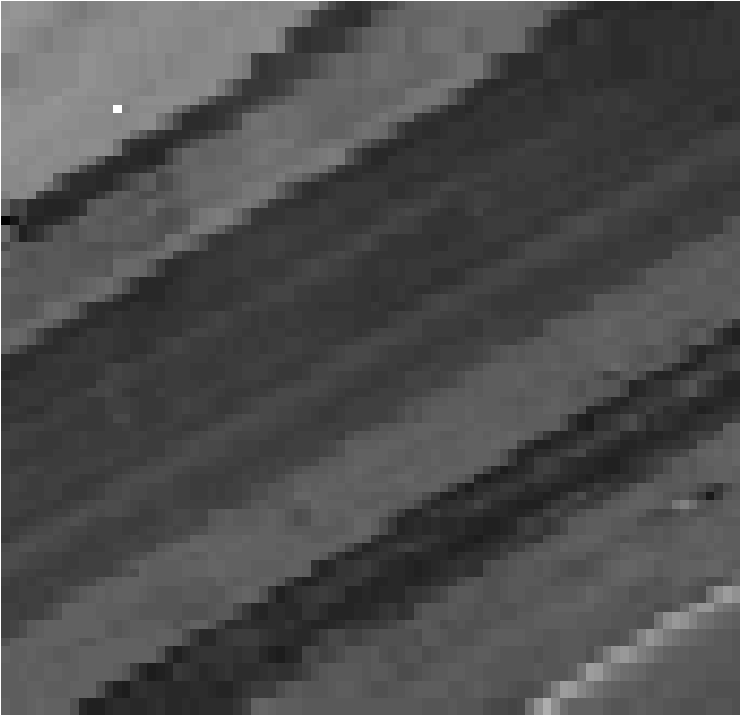
\includegraphics[width=.23\textwidth,clip]{Images/SalinasA_BandSum-crop.pdf}
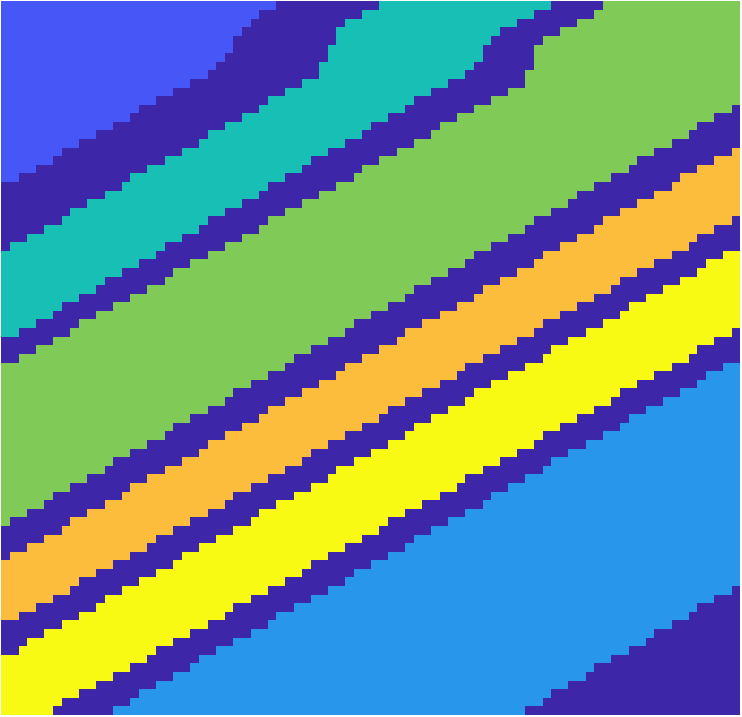
\includegraphics[width=.23\textwidth,clip]{Images/SalinasA_GT-crop.pdf}
\caption{\small{The $86\times 83$ Salinas A HSI data consists of 6 classes.  Left: the sum of all spectral bands.  Right: the ground truth.}}
\label{fig:SalinasA}
\end{figure}
The Salinas A HSI dataset of size $83 \times 86$ with $224$ spectral bands is represented as image of size $7138\times 224$. We use the unlabeled data to learn a latent space representation of Salinas A in $\R^{40}$ dimensions. The encoder network consists of three dense layers with $128$ units. The activation function is the rectified linear unit (RELU). The loss function is optimized using the Adam algorithm with learning rate set to $0.0001$. After training the VAE, we input the latent space representation of the Salinas A dataset to the LAND algorithm for the task of inferring the ground truth labels of the HSI data. We compare our result to the ``plain" LAND algorithm that simply clusters the Salinas A dataset in its original representation. Since LAND is an active learning framework, we consider varying number of labeled data points ranging from $10$ to $2000$. Figure \ref{fig:SalinasA} compares the performance of LAND and performance of VAE-LAND. First, for both VAE-LAND and standard LAND, LAND queries lead to significantly better accuracy than random queries. The proposed algorithm, VAE-LAND, attains an accuracy of 96.97\% with just 10 labeled points. This is a $12.5\%$ improvement to the accuracy of competitive LAND algorithm for the same number of labeled points. The standard LAND algorithm requires $400$ labeled points to reach accuracy of $90\%$ while for the same number of labeled points, VAE-LAND has an accuracy of $98.35\%$.  \JMM{Let's break down the model parameter description from the data description.} 

\begin{figure}
   % \centering
    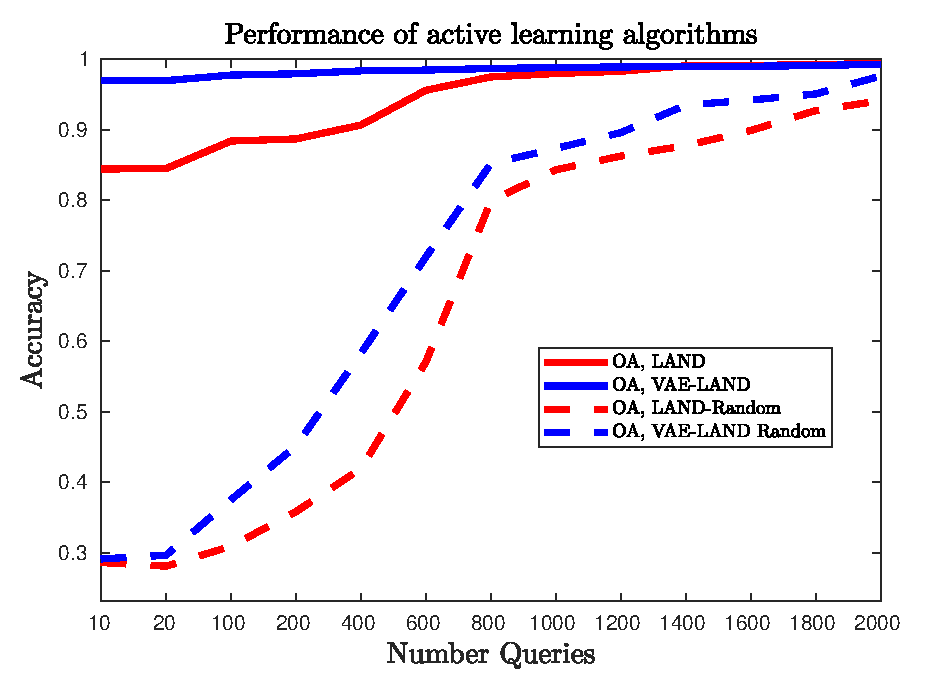
\includegraphics[width=.45\textwidth]{Images/salinasa_results_improved.eps}
    \caption{For the Salinas A dataset, the performance of variational autoencoder LAND learning achieves a higher accuracy than the standard LAND algorithm. With just $10$ points, the overall accuracy of VAE-LAND is 96.97\%, a 12.5\% improvement to the competitive LAND algorithm.  \JMM{Asymptotics?}}
    \label{fig:my_label}
\end{figure}

\subsection{Discussion of Experimental Results}



\subsection{Computational Complexity}



\section{Conclusions and Future Directions}
\label{sec:Conclusions}
The proposed active learning algortihm, VAE-LAND, improves over the standard LAND and gives accurate results even when the number of queries are limited. The method uses VAE to generate good features, and uses the diffusion geometry based LAND algorithm to determine query points. The LAND algorithm then uses this queried labels to predict the labels of the unlabeled data samples. In future work, we would like to explore the kind of data models for which the algorithm has theoretical performance guarantees.   
\section*{Acknowledgements}

This research is partially supported by the US National Science Foundation grants NSF-DMS 1912737, NSF-DMS 1924513, and NSF-CCF 1934553.




\bibliographystyle{IEEEbib}
\bibliography{IGARSS2021_ref}

\end{document}
